% !TeX root = statnicaEKT.tex
% !TeX spellcheck = sk_SK-Slovak
\part{BPC-AE1 - Analógová elektronika 1}
\begin{huge}
	Otázky:
	\newline
\end{huge}
\begin{enumerate}
	\item Otázka - Řízené zdroje. Imitanční invertor a konvertor. Ideální a reálný operační zesilovač. Proudový konvejor. Typická zapojení s operačním zesilovačem: napěťové a proudové zesilovače, převodníky. 
	\item Otázka - Analogové elektrické filtry: pasivní filtry prvního a druhého řádu, přenosové funkce, filtry vyšších řádů, typy aproximací, aktivní filtry (ARC).
	\item Otázka - Zesilovače: kritéria pro klasifikaci, základní parametry, třídy zesilovačů, účinnost, širokopásmové zesilovače, úzkopásmové (laděné) zesilovače, výkonové (koncové) nf zesilovače. 
\end{enumerate}
\newpage
\chapter{Riadené zdroje}
\section{Riadené zdroje}
Jedná sa o modely ideálnych dvojbranov používajúce sa k modelovaniu obvodov.
\begin{figure}[H]
	\centering
	\begin{subfigure}[b]{0.45\textwidth}
		\centering
		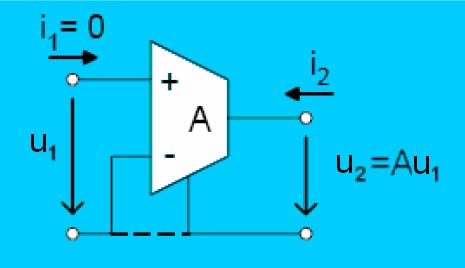
\includegraphics[width=0.7\linewidth]{Obrazky/AE1/VCVS}
		\caption[Riadené zdroje]{VCVS}
		\label{fig:VCVS}
	\end{subfigure}
	\begin{subfigure}[b]{0.45\textwidth}
		\centering
		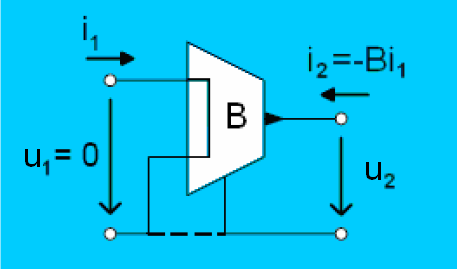
\includegraphics[width=0.7\linewidth]{Obrazky/AE1/CCCS}
		\caption[Riadené zdroje]{CCCS}
		\label{fig:CCCS}
	\end{subfigure}
	\begin{subfigure}[b]{0.45\textwidth}
		\centering
		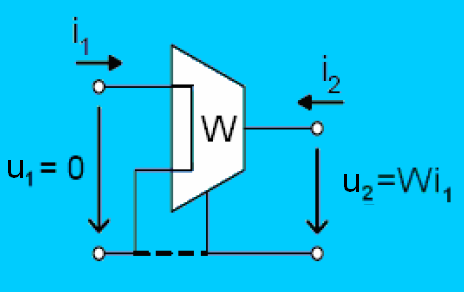
\includegraphics[width=0.7\linewidth]{Obrazky/AE1/CCVS}
		\caption[Riadené zdroje]{CCVS}
		\label{fig:CCVS}
	\end{subfigure}
	\begin{subfigure}[b]{0.45\textwidth}
		\centering
		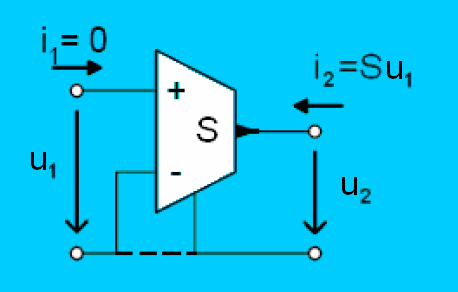
\includegraphics[width=0.7\linewidth]{Obrazky/AE1/VCCS}
		\caption[Riadené zdroje]{VCCS}
		\label{fig:VCCS}
	\end{subfigure}
	\caption{Štyri základné riadené zdroje}
	\label{fig:riadenezdroje}
\end{figure}
Popis k \ref{fig:riadenezdroje}
\begin{itemize}
	\item \ref{fig:VCVS} - Voltage Controled Voltage Source - Napäťovo riadený napäťový zdroj
	(Klasický OZ - OPA - Napäťový zosilňovač)
	\item \ref{fig:CCCS} - Current Controled Current Source - Prúdovo riadený prúdový zdroj
	(Prúdový zosilňovač)
	\item \ref{fig:CCVS} - Current Controled Voltage Source - Prúdovo riadený napäťový zdroj
	
	\item \ref{fig:VCCS} - Voltage Controled Current Source - Napäťovo riadený prúdový zdroj
	(Transkonduktančný zosilňovač - OTA)
\end{itemize}
\emph{Treba sa zamerať na jednotlivé prenosy a~značky blokov, ktoré sú vyznačené v obrázkoch na \ref{fig:riadenezdroje}}.

\section{Imitančný invertor a konvertor}
\subsubsection{Imitančný invertor}
Lineárny dvojbran. Jeho bránové prenosy sú viazané opačne, resp. inverzne. Prenosy sú nezávislé od vonkajšieho zapojenia.
\begin{figure}[H]
	\centering
	\begin{subfigure}[b]{0.65\textwidth}
		\centering
		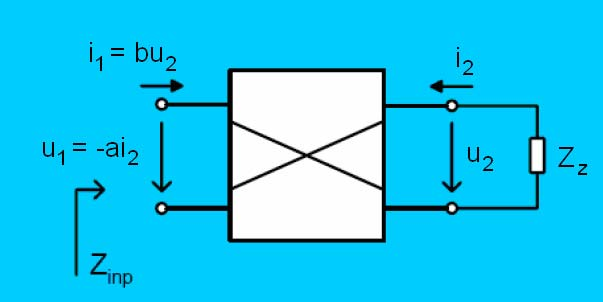
\includegraphics[width=0.6\linewidth]{Obrazky/AE1/imitInvert}
		\caption{Imitančný invertor}
		\label{fig:imitInvert}
	\end{subfigure}
	\begin{subfigure}[b]{0.3\textwidth}
		\centering
		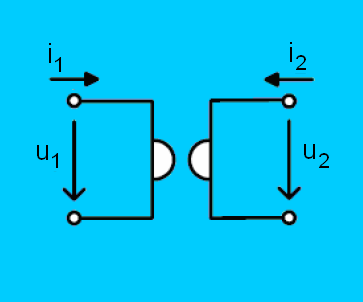
\includegraphics[width=0.7\linewidth]{Obrazky/AE1/gyrator}
		\caption{Špeciálny prípad Imitančného invertora - Gyrátor}
		\label{fig:gyrator}
	\end{subfigure}
	\label{fig:imitGyr}
	\caption{Imitančný invertor a gyrátor}
\end{figure}
Invertor transformuje zaťažovaciu impedanciu $Z_Z$ na vstupnú bránu, viz \ref{fig:imitInvert}. Pričom platí, že: 
\begin{equation}
	Z_{inp} = \frac{a}{b}\frac{1}{Z_Z} = k \cdot \frac{1}{Z_Z} \\
\end{equation}
Teda vstupná impedancia je úmerná inverznej hodnote zaťažovacej $Z_Z$. Podľa znamienka $k$, rozlišujeme medzi \emph{pozitívnym} a~\emph{negatívnym} invertorom $\implies$, \underline{$k > 0$ pozitívny, $k < 0$ negatívny invertor}.

\underline{Gyrátor \ref{fig:gyrator}, je pozitívny imitačný invertor} - Používa sa pri návrhu aktívnych RC filtrov a vyrába sa ako integrovaný obvod. Väčšinou býva symetrický.
Pri kapacitnej záťaži imituje induktívny charakter impedancie na vstupnej bráne. Pričom pre kapacitnú záťaž platí:
\begin{equation}
	Z_{inp} = k \cdot sC = s\cdot L_{ekv}
\end{equation}

\subsubsection{Imitačný konvertor}
Znovu lineárny dvojbran \ref{fig:imitKonvert}, Transformuje zaťažovaciu impedanciu na vstupnú bránu, s koeficientom $k$. Platí:
\begin{equation}
	Z_{inp} = \frac{a}{b}Z_Z = k \cdot Z_Z
\end{equation}
\begin{figure}[H]
	\centering
	\begin{subfigure}[b]{0.65\textwidth}
		\centering
		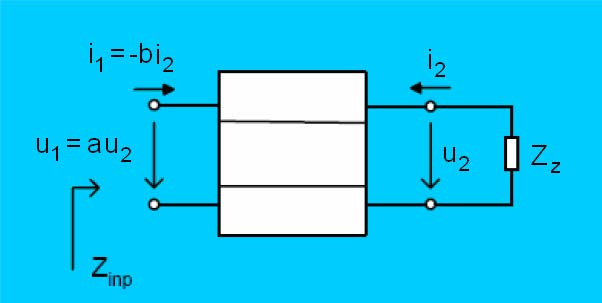
\includegraphics[width=0.6\linewidth]{Obrazky/AE1/imitKonvert}
		\caption{Imitančný konvertor}
		\label{fig:imitKonvert}
	\end{subfigure}
	\begin{subfigure}[b]{0.3\textwidth}
		\centering
		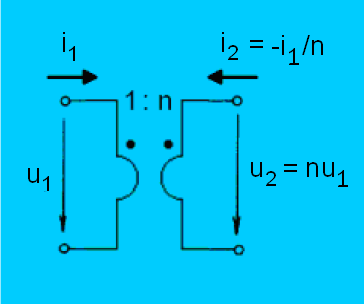
\includegraphics[width=0.7\linewidth]{Obrazky/AE1/idealTransform}
		\caption{Ideálny transformátor}
		\label{fig:idealTransform}
	\end{subfigure}
	\label{fig:konvTrans}
	\caption{Imitančný konvertor a ideálny transformátor}
\end{figure}

Podľa znamienka $k$, rozlišujeme medzi \emph{pozitívnym} \newline a~\emph{negatívnym} konvertorom $\implies$, \underline{$k > 0$ pozitívny, $k < 0$ negatívny konvertor}. Používa sa k získaniu záporného odporu. Prvok ako taký je neregurálny $\implies$ nedá sa popísať imitančnými parametrami (z imitančnej matice).

Obrázok \ref{fig:idealTransform} zobrazuje ideálny transformátor, čo je typ pozitívneho konvertora, kedy je zaťažovacia impedancia transformovaná na vstupnú bránu s kvadrátom, platí:
\begin{align}
	a &= \frac{1}{n} \\
	b &= n \\
	Z_{inp} &= \frac{1}{n^2} Z_Z
\end{align}

\section{Ideálny a reálny OZ}
\subsubsection{Ideálny OZ - (IOZ)}
Neregulárny dvojbran, považuje sa za limitný prípad ideálneho napäťového a prúdového zosilňovača, pričom zosilnenie ideálneho OZ je $\text{A} \rightarrow \infty$ a $\text{B} \rightarrow \infty$. Jeho vstupná impedancia je nekonečná a výstupná zase nulová. 

Podľa počtu vstupov vieme rozdeliť na:
\begin{description}
	\item[SISO] Single Input Single Output - nevyrába sa, realizuje sa z DISO - výstup skratneš s invertujúcim vstupom a vznikne buffer
	\item[DISO] Double Input Single Output - nazýva sa napäťový, najrozšírenejší OZ, všade ho dostať
	\item[SIDO] Single Input Double Output - duálne DISO, prúdový OZ, používa sa pre neivertujúci prúdový sledovač / zosilňovač
	\item[DIDO] Double Input Double Output - nazýva sa plávajúci, diferenciálny vstup a diferenciálny výstup, typický pre transimpedančný zosilňovač
\end{description}
\emph{Diferenciálny - symetrický, Single - nesymetrický}

\subsubsection{Reálny OZ}
Reálny OZ má obmedzené hodnoty zosilnenia, $A_0 \approx 10^5$, jeho vstupná impedancia je rovnako konečná, pričom výstupná je nenulová. Nakoľko sa jedná o reálnu štruktúru, má aj parazitné javy:
\begin{multicols}{2}
	\begin{itemize}
		\item offset, medzi vstupmi $U_{IO}$, závisí na teplotnom a časovom drifte či na prieniku napájacieho napätia - jeho kolísaniu
		\item prúdová nesymetria vstupov,
		\item vstupný odpor (impedancia),
		\item frekvenčná závislosť zosilnenia $A$,
		\item drift (utekanie $U_{IO}$),
		\item vstupné zvyškové prúdy,
		\item výstupný odpor (impedancia).
	\end{itemize}
\end{multicols}

Pri OZ sa udáva frekvenčná (modulová) a pracovná charakteristika. \newline
\underline{Pracovná charakteristika \ref{fig:pracovnaChar}}
Vzťah medzi vstupným a výstupným napätím - strmosť predstavuje zosilnenie. Obsahuje okrajové časti - vrchná a spodná limitácia (saturácia z napájacieho napätia), a stredná časť - aktívna oblasť. Stred aktívnej oblasti neprechádza nulou ale prechádza offsetom / nesymetriou.

\underline{Modulová charakteristika \ref{fig:modulChar}}
Štandardná charakteristika udaná jedným pólom, odpovedá prenosovej funkcii:
\begin{equation}
	A(s) = \frac{A_0 \omega_0}{s + \omega_0}
\end{equation}
Pričom $\omega_0$ odpovedá \qty{-3}{\dB} - teda je to \underline{medzná frekvencia}, $\omega_t$ je \underline{tranzientná frekvencia} - keď zisk $A = 0 \; \unit{dB}$.

\begin{figure}[H]
	\centering
	\begin{subfigure}[b]{0.45\textwidth}
		\centering
		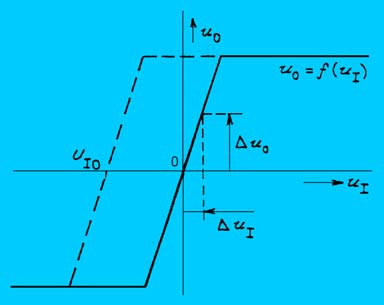
\includegraphics[width=0.7\linewidth]{Obrazky/AE1/pracovnaChar}
		\caption{Pracovná charakteristika OZ}
		\label{fig:pracovnaChar}
	\end{subfigure}
	\begin{subfigure}[b]{0.45\textwidth}
		\centering
		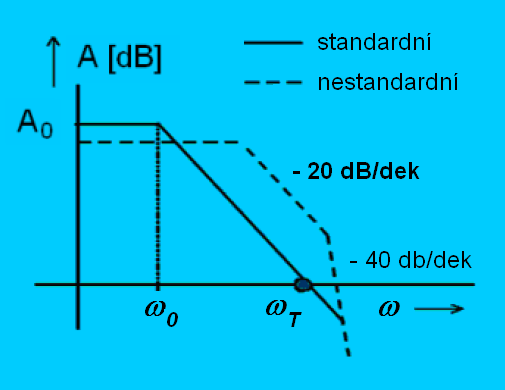
\includegraphics[width=0.7\linewidth]{Obrazky/AE1/modulchar}
		\caption{Modulová charakteristika OZ}
		\label{fig:modulChar}
	\end{subfigure}
	\label{fig:OZChar}
	\caption{Charakteristiky OZ}
\end{figure}

\section{Prúdový konvejor}
Funkčné mnohobrany, ktorých vzťahy sú medzi bránami sú rôzne definované bránovými veličinami. \underline{Konvejorovaním} sa rozumie sledovanie U a I, je možná aj inverzia. Konvejor \ref{fig:konvejor} dosahuje lepšie frekvenčné vlastnosti ako štandardný OZ - pracuje v prúdovom móde.
\begin{figure}[htpb]
	\centering
	% --- ĽAVÁ STRANA: OBRÁZOK ---
	\begin{minipage}[c]{0.35\textwidth}
		\centering
		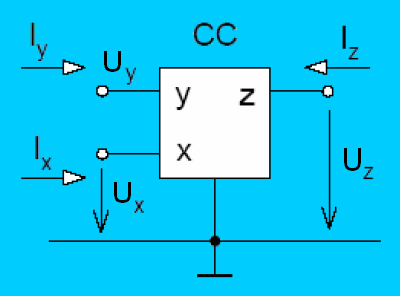
\includegraphics[width=\linewidth]{Obrazky/AE1/konvejor}
		\caption{Trojbránový konvejor typu CCII+}
		\label{fig:konvejor}
	\end{minipage}
	\hfill % Vyplní medzeru medzi minipages
	% --- PRAVÁ STRANA: TEXT A ROVNICE ---
	\begin{minipage}[c]{0.60\textwidth}
		Pre vzťahy medzi bránovými veličinami platí:
		\begin{align*}
			U_x &= U_y \\
			I_y &= 0 \\
			I_z &= I_x 
		\end{align*}
		Obecne platí:
		\begin{equation*}
			\begin{aligned}
				U_x &= aU_y \\
				I_y &= bI_x \\
				I_z &= cI_x 
			\end{aligned}
			\,\implies\,
			\begin{pmatrix} U_x \\ I_y \\ I_z \end{pmatrix} = 
			\begin{pmatrix} 
				a & 0 & 0 \\ 
				0 & b & 0 \\ 
				0 & c & 0 
			\end{pmatrix} 
			\begin{pmatrix} U_y \\ I_x \\ I_x \end{pmatrix}
		\end{equation*}
	\end{minipage}
\end{figure}
\subsubsection{Rozdelenie Konvejorov}
\emph{Asi netreba ale len pre úplnosť}
\begin{description}
	\item[Koeficient $a = \{+1, -1\}$] (Smer/polarita prenosu napätia)
	\begin{description}
		\item[$+1$:] \textbf{CC (neinvertujúci)} -- napätie sa prenáša bez zmeny polarity.
		\item[$-1$:] \textbf{ICC (invertujúci)} -- napätie sa na výstupe invertuje.
	\end{description}
	
	\item[Koeficient $b = \{+1, 0, -1\}$] (Generácie prúdových konvejorov)
	\begin{description}
		\item[$+1$:] \textbf{CCI (1. generácia, 1968)} -- prvá verzia prúdového konvejoru.
		\item[$\phantom{+}0$:] \textbf{CCII (2. generácia, 1970)} -- druhá, najpoužívanejšia generácia (autori Sedra \& Smith).
		\item[$-1$:] \textbf{CCIII (3. generácia, 1995)} -- tretia generácia (autor Fabre).
	\end{description}
	
	\item[Koeficient $c = \{+1, -1\}$] (Smer/polarita výstupného prúdu)
	\begin{description}
		\item[$+1$:] \textbf{CC+ (pozitívny)} -- výstupný prúd tečie rovnakým smerom (pozitívna polarita).
		\item[$-1$:] \textbf{CC- (negatívny)} -- výstupný prúd tečie opačným smerom (negatívna polarita).
	\end{description}
\end{description}

\section{Typické zapojenia s OZ}
\subsubsection{Zapojenia s napäťovým zosilňovačom}
\begin{figure}[H]
	\centering
	\begin{subfigure}[b]{0.45\textwidth}
		\centering
		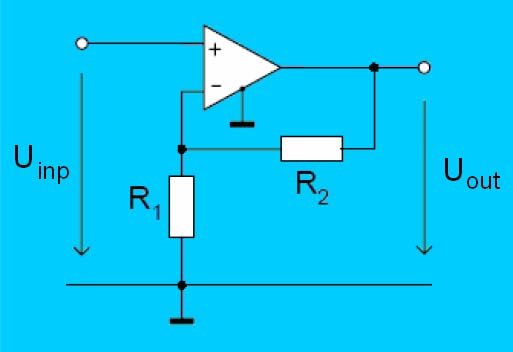
\includegraphics[width=0.6\linewidth]{Obrazky/AE1/zosikPlus}
		\caption{Neinvertujúci zosilňovač}
		\label{fig:zos}
	\end{subfigure}
	\begin{subfigure}[b]{0.45\textwidth}
		\centering
		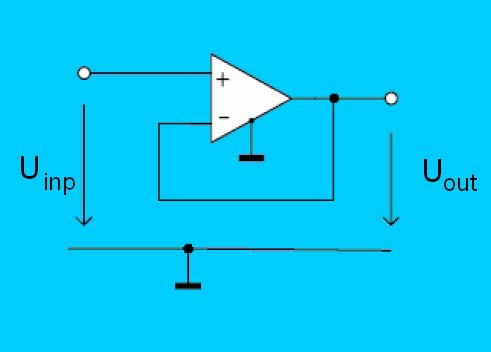
\includegraphics[width=0.6\linewidth]{Obrazky/AE1/buufer}
		\caption{Buffer - sledovač}
		\label{fig:buffer}
	\end{subfigure}
	\begin{subfigure}[b]{0.45\textwidth}
		\centering
		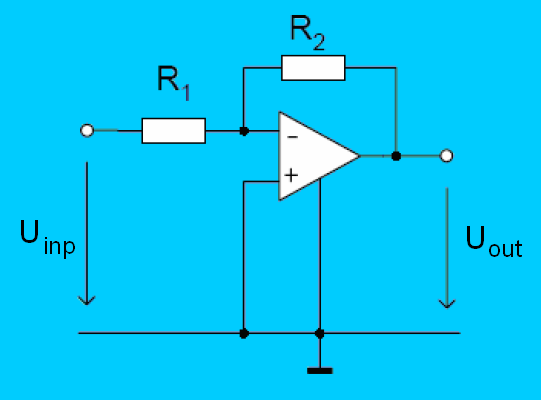
\includegraphics[width=0.6\linewidth]{Obrazky/AE1/zosikMinus}
		\caption{Invertujúci zosilňovač}
		\label{fig:zosInvert}
	\end{subfigure}
	\begin{subfigure}[b]{0.45\textwidth}
		\centering
		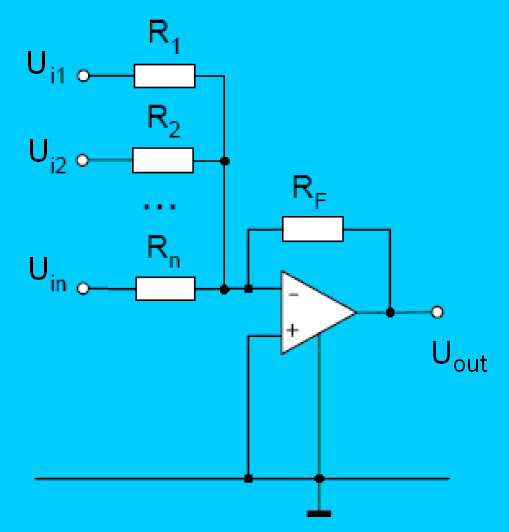
\includegraphics[width=0.5\linewidth]{Obrazky/AE1/sumator}
		\caption{Sumačný zosilňovač}
		\label{fig:sumator}
	\end{subfigure}
	\caption{Štyri základné zapojenia s Napäťovým OZ}
	\label{fig:zapojeniaNapatoveOZ}
\end{figure}
Na obrázku \ref{fig:zapojeniaNapatoveOZ} sú uvedené typické zapojenie s využitím napäťového zosilňovača. Pre neinvertujúci zosilňovač, obrázok \ref{fig:zos}, platí prenos:
	\begin{align*}
		\text{Ideálny prípad } (A \to \infty): \quad K_U &= 1 + \frac{R_2}{R_1} 
		& 
		\text{Reálny OZ: } \quad K_U &= \frac{A(R_1 + R_2)}{R_1(A + 1) + R_2}
	\end{align*}
Modifikáciou na buffer (vytvoríme SISO) obrázok \ref{fig:buffer}, dosiahneme: 
\begin{equation*}
	K_U = \frac{U_{out}}{U_{in}} = 1
\end{equation*}
Inverujúci napäťový zosilňovač, obrázok \ref{fig:zosInvert}:
\begin{align}
	\text{Ideálny prípad: } \quad K_U &= -\frac{R_2}{R_1} 
	& 
	\text{Reálny OZ: } \quad K_U &= \frac{-AR_2}{R_1(A + 1) + R_2}
	\label{eqv:invertOZPrenos}
\end{align}
Kedy narozdiel od prechádzajúcich zapojení je pri \ref{fig:zosInvert}, vstupná impedancia daná $R_1$ a prúd na vstupne je nenulový.

Obrázky \ref{fig:zos}, \ref{fig:buffer} a \ref{fig:zosInvert}. Boli asi veľmi jednoduché tak si niekto vymyslel sumátor napätia, obrázok \ref{fig:sumator}. Výstup je daný:
\begin{equation}
	U_{out} = - \left( \frac{R_F}{R_1} U_{i1} + \frac{R_F}{R_2} U_{i2} + \dots + \frac{R_F}{R_n} U_{in} \right)
\end{equation}
\emph{Existujú aj zložitejšie zapojenia s využitím rozsiahlejších odporových sietí, každé má inú prenosovú funkciu.}

\subsubsection{Zapojenia s prúdovým zosilňovačom}
Prúdový zosilňovač sa dá vytvoriť výmenou vstupov za výstupy pri DISO - vieme tak dosiahnuť SIDO. V obvodoch je realizovaná záporná prúdová paralelná spätná väzba (Delič $R_1$ a $R_2$ v obrázku \ref{fig:zosPrud}), teda časť vstupného prúdu sa privádza do výstupnej brány.
\begin{figure}[H]
	\centering
	\begin{subfigure}[b]{0.45\textwidth}
		\centering
		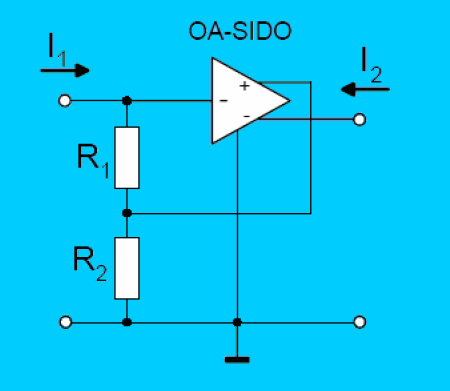
\includegraphics[width=0.55\linewidth]{Obrazky/AE1/zosPrud}
		\caption{Prúdový zosilňovač}
		\label{fig:zosPrud}
	\end{subfigure}
	\begin{subfigure}[b]{0.45\textwidth}
		\centering
		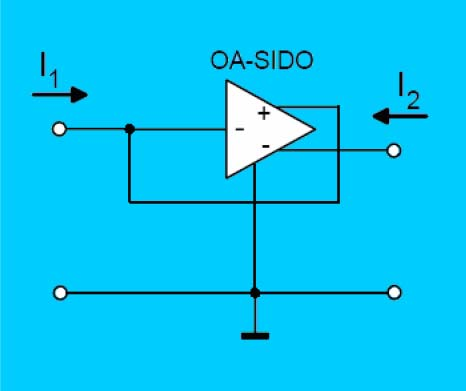
\includegraphics[width=0.55\linewidth]{Obrazky/AE1/bufferPrud}
		\caption{Prúdový sledovač}
		\label{fig:bufferPrud}
	\end{subfigure}
	\label{fig:zapojeniaPrudove}
	\caption{Zapojenia prúdových zosilňovačov}
\end{figure}
Platí: 
\begin{equation}
	K_I = \frac{-I_2}{I_1} = 1 + \frac{R_1}{R_2}
\end{equation}
Jedná sa o duálny vzťah k \ref{eqv:invertOZPrenos}. Rovnako je vstupná impedancia nulová a teda aj vstupné napätie???

\subsubsection{Prevodník prúd - napätie}
\begin{figure}[H]
	\centering
	% --- ĽAVÁ STRANA: OBRÁZOK ---
	\begin{minipage}[c]{0.35\textwidth}
		\centering
		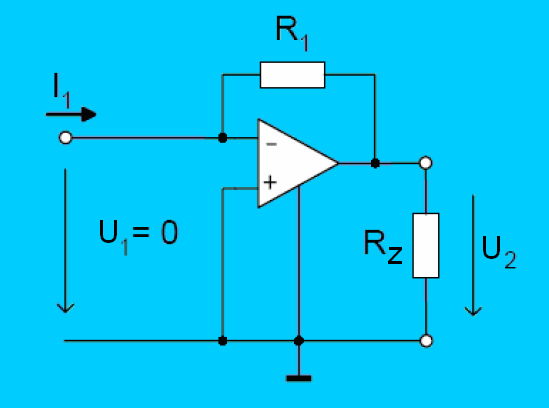
\includegraphics[width=\linewidth]{Obrazky/AE1/prevodnikUI}
		\caption{Prevodník prúdu na napätie}
		\label{fig:prevodnikIU}
	\end{minipage}
	\hfill % Vyplní medzeru medzi minipages
	% --- PRAVÁ STRANA: TEXT A VZORCE ---
	\begin{minipage}[c]{0.60\textwidth}
		Zapojenie na obrázku \ref{fig:prevodnikIU} sa nazýva prevodník prúd -- napätie, alebo aj transrezistor (má tzv. transimpedanciu $Z_T$). Dá sa realizovať aj z SISO. Pre transimpedanciu $Z_T$ tohto prevodníka platí:
		
		\begin{align*}
			\text{Reálny OZ: } \ Z_T &= \frac{U_2}{I_1} = -\frac{R_1 A}{1 + A} \\
			\text{Ideálny OZ } (A \to \infty): \ Z_T &= \frac{U_2}{I_1} = -R_1
		\end{align*}
	\end{minipage}
\end{figure}
\subsubsection{Prevodník napätie - prúd}
Nazýva sa transkonduktor, jeho realizácia záleží od typu záťaže - oddelená či zemnená.
\begin{figure}[H]
	\centering
	\begin{subfigure}[b]{0.45\textwidth}
		\centering
		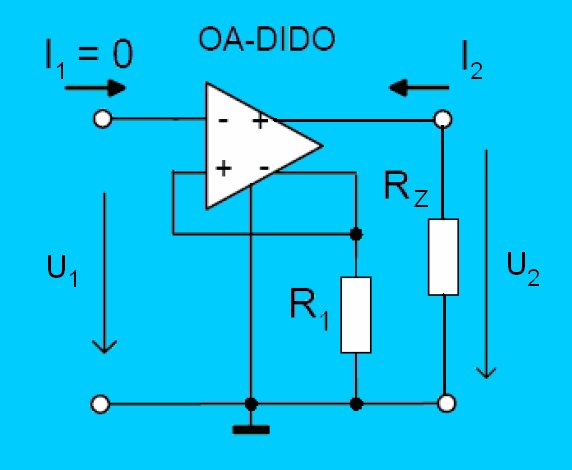
\includegraphics[width=0.55\linewidth]{Obrazky/AE1/didoUI}
		\caption{U/I prevodník s DIDO}
		\label{fig:prevodnikUIdido}
	\end{subfigure}
	\begin{subfigure}[b]{0.45\textwidth}
		\centering
		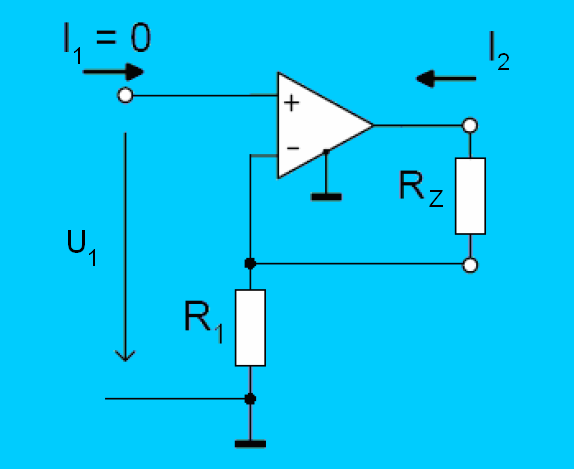
\includegraphics[width=0.55\linewidth]{Obrazky/AE1/disoUI}
		\caption{U/I prevodník s DISO}
		\label{fig:prevodnikUIdiso}
	\end{subfigure}
	\label{fig:zapojeniaUIprevodnikov}
	\caption{Zapojenia prevodníkov napätie - prúd}
\end{figure}
Obvod má nasledujúce parametre:
\begin{equation}
	I_1 = 0 \quad \text{(a)}, \qquad -I_2 = Y_T U_1 \quad \text{(b)}, \qquad Y_T = \frac{-I_2}{U_1} = -\frac{1}{R_1} \quad \text{(c)}
\end{equation}

Prevodník $U \to I$ s plávajúcou záťažou ($R_Z$) je možné jednoduchšie realizovať s OZ-DISO. Pre transkonduktanciu $Y_T$ tohto prevodníka platí:

\begin{align*}
	\text{Reálny OZ: } \quad Y_T &= \frac{-I_2}{U_1} = \frac{A}{R_Z + R_1(1 + A)}
	&
	\text{Ideálny prípad } (A \to \infty): \quad Y_T &= \frac{1}{R_1}
\end{align*}

Vstupná a výstupná impedancia oboch vyššie uvedených transkonduktorov sú v ideálnom prípade nekonečné.
\newpage
\chapter{Analógové elektrické filtre}
Frekvenčné filtre sú lineárne dvojbrany. Ich účel je jasný - prepustia len isté frekvenčné pásmo, zvyšné pásmo je potláčané. Filtre sa delia podľa:
\begin{itemize}
	\item prenášanáho pásma (Dolná priepusť, Horná priepusť, Pásmová priepusť, Pásmová zádrž)
	\item tvaru frekvenčnej charakteristiky
	\item rádu prenosovej funkcie
	\item použitých prvkov (RC, LC/RLC, aktívne R, syntetické (s gyrátorom), SAW)
\end{itemize}


\section{Pasívne filtre}
\subsubsection{Prvého rádu}
Pasívne filtre sú v podstate frekvenčne závislé deliče - teda v najzákladnejšej podobe (RC, CR 1. rádu)

\begin{figure}[H]
	\centering
	\begin{subfigure}[b]{0.45\textwidth}
		\centering
		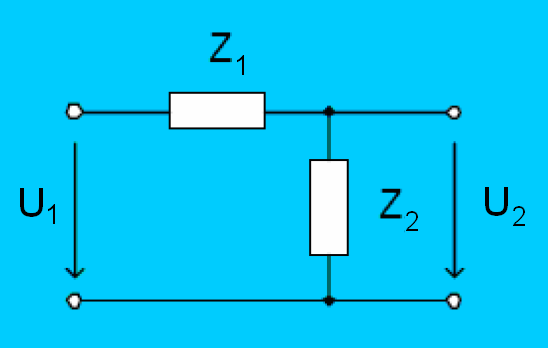
\includegraphics[width=0.6\linewidth]{Obrazky/AE1/druhaOtazka/frekZZ}
		\caption{Frekvenčne závislý delič napätia}
		\label{fig:frekZZ}
	\end{subfigure}
	\begin{subfigure}[b]{0.45\textwidth}
		\centering
		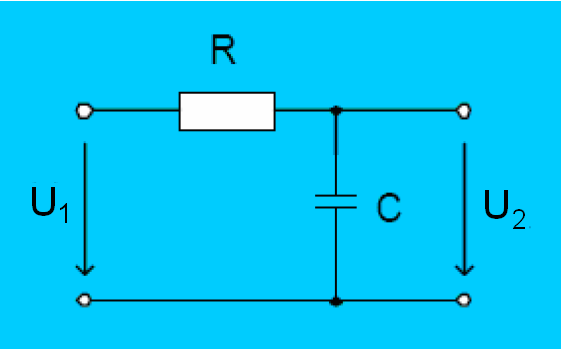
\includegraphics[width=0.6\linewidth]{Obrazky/AE1/druhaOtazka/RC}
		\caption{RC filter - 1 rád - dolná priepusť}
		\label{fig:RC}
	\end{subfigure}
	\begin{subfigure}[b]{0.45\textwidth}
		\centering
		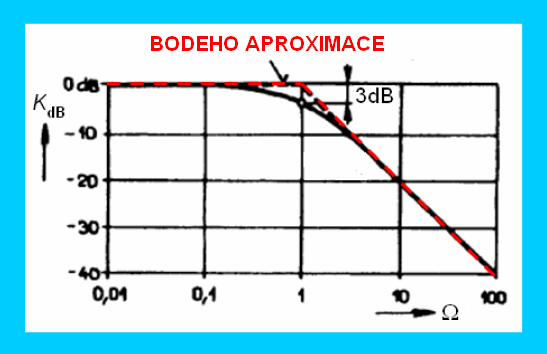
\includegraphics[width=0.6\linewidth]{Obrazky/AE1/druhaOtazka/RCfrek}
		\caption{Frekvenčná / Modulová charakteristika}
		\label{fig:RCfrek}
	\end{subfigure}
	\begin{subfigure}[b]{0.45\textwidth}
		\centering
		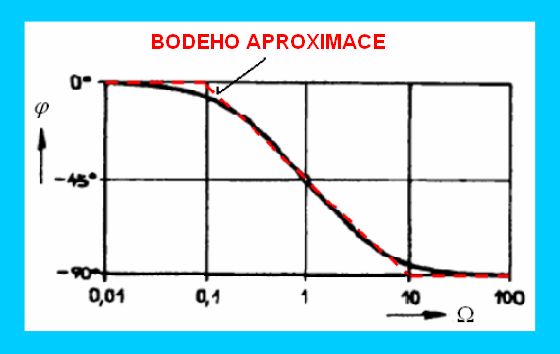
\includegraphics[width=0.6\linewidth]{Obrazky/AE1/druhaOtazka/RCfaza}
		\caption{Fázová / Argumentová charakteristika}
		\label{fig:RCfaza}
	\end{subfigure}
	\caption{Základný polčlánok - frekvenčne závislý delič}
	\label{fig:RCpvehoradu}
\end{figure}
Uvažujme dolný priepust RC ako príklad pasívneho filtra 1. rádu. Po dosadení za príslušné impedancie dostávame pre prenosovú funkciu vzťah:
\begin{equation}
	\mathbf{K}(j\omega) = \frac{1 / j\omega C}{R + 1 / j\omega C} = \frac{1}{1 + j\omega RC}
\end{equation}

Modulová charakteristika \ref{fig:RCfrek} tohto obvodu je potom daná vzťahom:
\begin{equation}
	K(\omega) = |\mathbf{K}(j\omega)| = \frac{1}{\sqrt{1 + \omega^2 R^2 C^2}}
\end{equation}

Zisk v decibeloch je rovný:
\begin{equation}
	k(\omega) = K_{\text{dB}}(\omega) = 20 \log K(\omega)
\end{equation}

Argumentová (fázová) \ref{fig:RCfaza} charakteristika je daná vzťahom:
\begin{equation}
	\varphi(\omega) = \arg \mathbf{K}(j\omega) = -\arctan \omega RC
\end{equation}
Medzný kmitočet $\omega_m$ je definovaný poklesom zisku o \SI{-3}{dB} (argument je rovný \SI{-45}{^\circ}):
\begin{equation}
	K(\omega_m) = \frac{K_0}{\sqrt{2}} \quad (\text{kde } K_0 = 1), \qquad K_{\text{dB}}(\omega_m) = K_{0\text{dB}} - 3
\end{equation}

V tomto obvode je daný vzťahom:
\begin{equation}
	\omega_m = \frac{1}{\tau} = \frac{1}{RC} \implies f_m = \frac{1}{2 \pi \cdot R C}
\end{equation}

Na medznom kmitočte nastáva zmena v sklone asymptot pri Bodeho aproximácii modulovej charakteristiky (s maximálnou odchýlkou \SI{3}{dB} od skutočnej). Pri fázovej charakteristike sú zlomy dva (dekádu pred a dekádu po $\omega_m$, s maximálnou odchýlkou \SI{5.7}{^\circ}).

Pre jednoduchší návrh zavádzame normované kmitočtové premenné:
\begin{equation}
	p = \frac{s}{\omega_N}, \qquad \Omega = \frac{\omega}{\omega_N}
\end{equation}

Najčastejšie normujeme k medznému kmitočtu $\omega_N = \omega_m$. Obvodové funkcie dolného priepustu 1. rádu sú potom v normovanom tvare:
\begin{equation}
	K(p) = \frac{1}{1 + p}, \qquad K(\Omega) = \frac{1}{\sqrt{1 + \Omega^2}}, \qquad \varphi(\Omega) = -\arctan\Omega
\end{equation}
\subsubsection{Druhého rádu}
Vyššiu strmosť frekvenčnej charakteristiky \ref{fig:RCfrek} vieme dosiahnuť zvýšením rádu filtra. Pre \ref{fig:RC} to dosiahneme náhradou R za L - vznikne R + L v sérií, R vyjadruje straty na L, dostaneme dolnú prepusť 2. rádu. Prenosové funkcie vyzerajú nasledovne:
Pre tento obvod je možné odvodiť napäťový prenos vo všeobecnom tvare:
\begin{equation}
	K(s) = \frac{a_0}{b_2 s^2 + b_1 s + b_0} = \frac{K_0}{LCs^2 + RCs + 1} = \frac{K_0 \omega_p^2}{s^2 + \frac{\omega_p}{Q_p} s + \omega_p^2}
\end{equation}

Póly sú komplexne združené ($\operatorname{Im} p_1 = -\operatorname{Im} p_2$), ich frekvencia je:
\begin{equation}
	\omega_p = \frac{1}{\sqrt{LC}}
\end{equation}

a činiteľ kvality je daný vzťahom (činiteľ kvality hovorí o veľkosti prekmitu na lomovej frekvencii):
\begin{equation}
	Q_p = \frac{\omega_p}{2\sigma_p} = \frac{\omega_p L}{R}
\end{equation}

Uhlová frekvencia $\omega_d$, vyznačená na imaginárnej osi, vyjadruje vlastný kmitočet oscilácií.

% --- PRENOSOVÉ FUNKCIE VEDĽA SEBA ---
\begin{align*}
	\text{Dolná priepust (LP): } \quad K(s) &= \frac{K_0 \omega_p^2}{s^2 + \frac{\omega_p}{Q_p} s + \omega_p^2}
	&
	\text{Horná priepust (HP): } \quad K(s) &= \frac{K_0 s^2}{s^2 + \frac{\omega_p}{Q_p} s + \omega_p^2}
\end{align*}
Hornú priepusť 2. rádu vieme realizovať zámenou C za R + L.
\begin{figure}[H]
	\centering
	\begin{subfigure}[b]{0.28\textwidth}
		\centering
		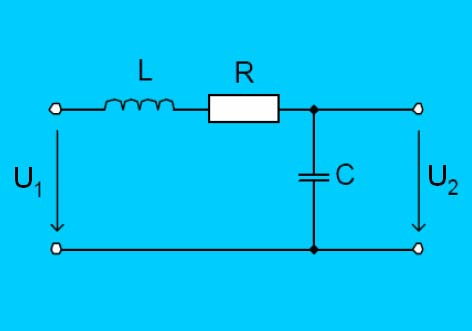
\includegraphics[width=0.8\linewidth]{Obrazky/AE1/druhaOtazka/LRC}
		\caption{Dolná priepusť 2. rádu}
		\label{fig:LRC}
	\end{subfigure}
	\begin{subfigure}[b]{0.28\textwidth}
		\centering
		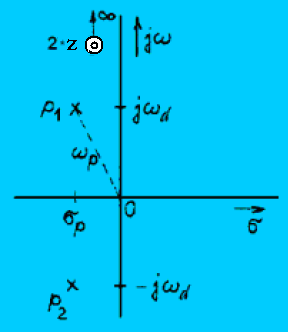
\includegraphics[width=0.55\linewidth]{Obrazky/AE1/druhaOtazka/LRCnula}
		\caption{rozloženie pólov a núl}
		\label{fig:LRCnula}
	\end{subfigure}
	\begin{subfigure}[b]{0.28\textwidth}
		\centering
		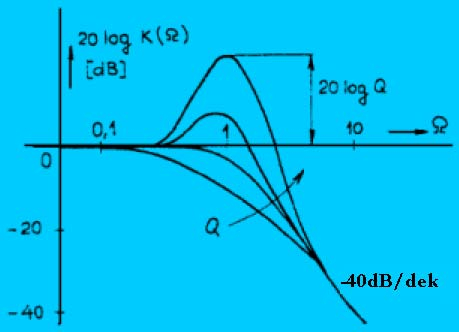
\includegraphics[width=0.8\linewidth]{Obrazky/AE1/druhaOtazka/LRCmodul}
		\caption{modulová charakteristika}
		\label{fig:LRCmodul}
	\end{subfigure}
	\label{fig:LRCdolna}
	\caption{Dolná priepusť 2. rádu}
\end{figure}
\begin{figure}[H]
	\centering
	\begin{subfigure}[b]{0.28\textwidth}
		\centering
		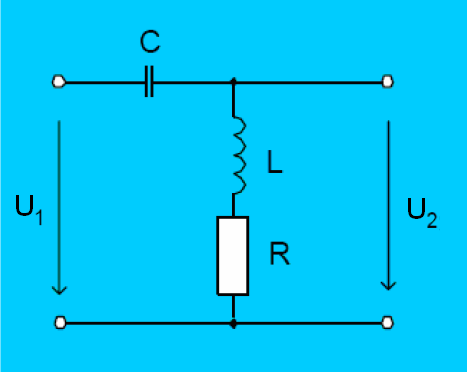
\includegraphics[width=0.8\linewidth]{Obrazky/AE1/druhaOtazka/CLR}
		\caption{Horná priepusť 2. rádu}
		\label{fig:CLR}
	\end{subfigure}
	\begin{subfigure}[b]{0.28\textwidth}
		\centering
		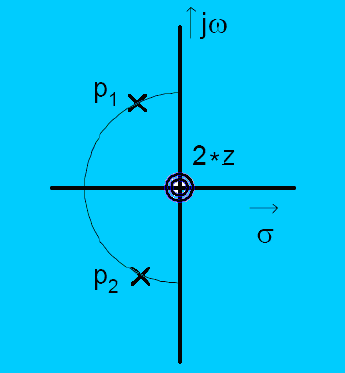
\includegraphics[width=0.55\linewidth]{Obrazky/AE1/druhaOtazka/CLRnula}
		\caption{rozloženie pólov a núl}
		\label{fig:CLRnula}
	\end{subfigure}
	\begin{subfigure}[b]{0.28\textwidth}
		\centering
		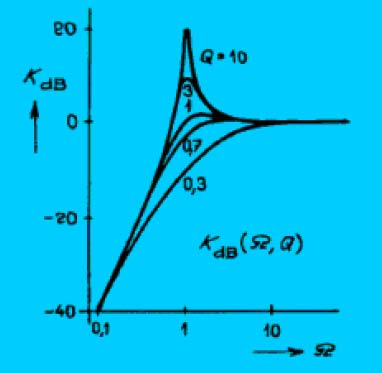
\includegraphics[width=0.8\linewidth]{Obrazky/AE1/druhaOtazka/CLRmodul}
		\caption{modulová charakteristika}
		\label{fig:CLRmodul}
	\end{subfigure}
	\label{fig:CLRhorna}
	\caption{Horná priepusť 2. rádu}
\end{figure}
\subsubsection{Pásmové Priepuste / Zádrže}
\begin{figure}[H]
	\centering
	\begin{subfigure}[b]{0.28\textwidth}
		\centering
		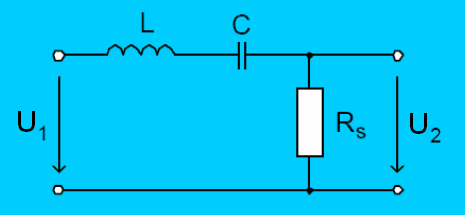
\includegraphics[width=0.8\linewidth]{Obrazky/AE1/druhaOtazka/PPRS}
		\caption{Realizácia pásmovej priepuste 2. rádu}
		\label{fig:PPRS}
	\end{subfigure}
	\begin{subfigure}[b]{0.28\textwidth}
		\centering
		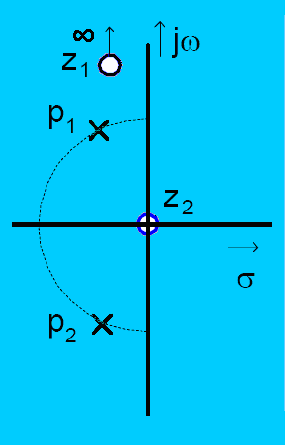
\includegraphics[width=0.55\linewidth]{Obrazky/AE1/druhaOtazka/PPnula}
		\caption{rozloženie pólov a núl}
		\label{fig:PPnula}
	\end{subfigure}
	\begin{subfigure}[b]{0.28\textwidth}
		\centering
		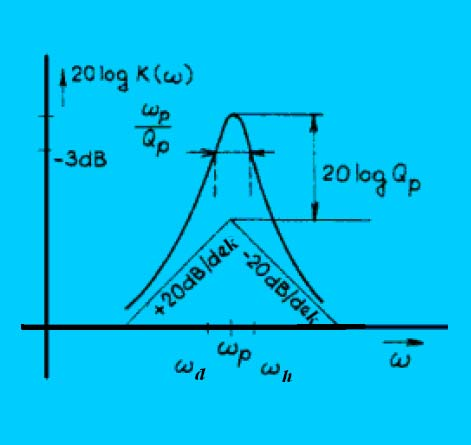
\includegraphics[width=0.8\linewidth]{Obrazky/AE1/druhaOtazka/PPmodul}
		\caption{modulová charakteristika}
		\label{fig:PPmodul}
	\end{subfigure}
	\label{fig:PP}
	\caption{Pásmová priepusť 2. rádu}
\end{figure}
\begin{figure}[H]
	\centering
	\begin{subfigure}[b]{0.28\textwidth}
		\centering
		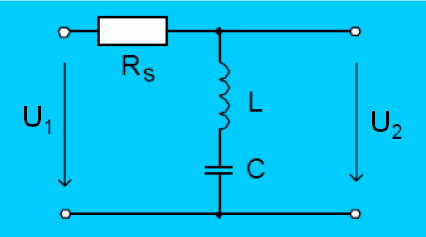
\includegraphics[width=0.8\linewidth]{Obrazky/AE1/druhaOtazka/PZRS}
		\caption{Pásmová zádrž 2. rádu}
		\label{fig:PZRS}
	\end{subfigure}
	\begin{subfigure}[b]{0.28\textwidth}
		\centering
		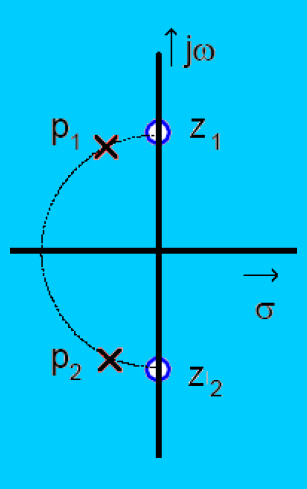
\includegraphics[width=0.55\linewidth]{Obrazky/AE1/druhaOtazka/PZnula}
		\caption{rozloženie pólov a núl}
		\label{fig:PZRSnula}
	\end{subfigure}
	\begin{subfigure}[b]{0.28\textwidth}
		\centering
		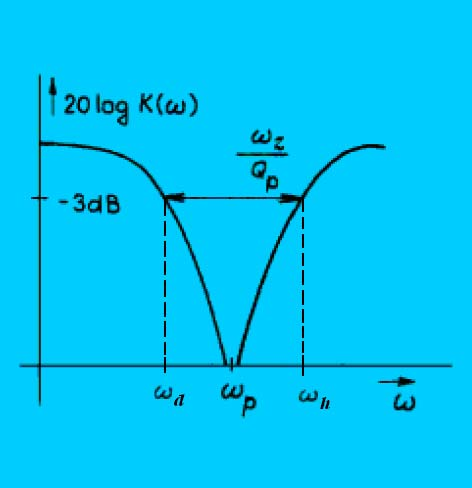
\includegraphics[width=0.8\linewidth]{Obrazky/AE1/druhaOtazka/PZmodul}
		\caption{modulová charakteristika}
		\label{fig:PZRSmodul}
	\end{subfigure}
	\caption{Pásmová zádrž 2. rádu}
	\label{fig:PZ}
\end{figure}
Prenosová funkcia pásmovej priepuste (PP) a pásmovej zádrže (PZ) vo všeobecnom tvare:
\begin{align*}
	\text{Pásmová priepusť (PP): } \quad K(s) &= \frac{a_1 s}{b_2 s^2 + b_1 s + b_0} = \frac{K_0 \frac{\omega_p}{Q_p} s}{s^2 + \frac{\omega_p}{Q_p} s + \omega_p^2} \\
	\text{Pásmová zádrž (PZ): } \quad K(s) &= \frac{a_2 s^2 + a_0}{b_2 s^2 + b_1 s + b_0} = K_0 \frac{s^2 + \omega_p^2}{s^2 + \frac{\omega_p}{Q_p} s + \omega_p^2} \quad \Longleftarrow \quad \omega_z = \omega_p
\end{align*}
Parametre pásmovej priepuste (PP) sú dané nasledovne:
\begin{equation}
	\omega_p = \omega_{\text{rez}} = \frac{1}{\sqrt{LC}}, \qquad Q_p = \frac{\omega_p L}{R_s} = \frac{R_p}{\omega_p L},\qquad B_\omega = \omega_h - \omega_d = \frac{\omega_p}{Q_p}
\end{equation}
\underline{Všeobecný obvod 2. rádu sa nazýva bikvád - bikvadratická štruktúra.} Jeho prenosová funkcia je nižšie. Platí, že $\omega_p = \omega_z$. Teda Póly a Nuly ležia v imaginárnej rovine na jednej kružnici \ref{fig:PZRSnula}. Pásmová zádrž \ref{fig:PZ} spĺňa podmienky pre bikvád.
\begin{equation}
	K(s) = \frac{a_2 s^2 + a_1 s + a_0}{b_2 s^2 + b_1 s + b_0} = K_0 \frac{(s - z_1)(s - z_2)}{(s - p_1)(s - p_2)} = K_0 \frac{s^2 + \frac{\omega_z}{Q_z} s + \omega_z^2}{s^2 + \frac{\omega_p}{Q_p} s + \omega_p^2} \ .
\end{equation}
Existuje aj všepriepustný obvod - fázovací bikvád. Jeho modul je konštantný. Body Nuly a Pólov sú v pravej polovici imaginárnej roviny. Fáza sa s frekvenciou mení.

\section{Aktívne filtre}
Nazývajú sa ARC, majú mnohé usporiadania, pasívne prvky RLC nahradzujú zapojením RC s operačným zosilňovačom. Existujú mnohé topológie aktívnych filtrov. Základným stavebným blokom sú bikvadické štruktúry / topológie ARC. Vieme ich rozlíšiť v závislosti od usporiadania spätnej väzby:
\begin{multicols}{2}
\begin{itemize}
	\item jedna slučka ZV
	\item dve slučky ZV
	\item viacero slučiek ZV
	\item priečkový článok RC
	\item T-článok RC
	\item Wienov článok RC
\end{itemize}
\end{multicols}
\begin{figure}[H]
	\begin{subfigure}[b]{0.45\textwidth}
		\centering
		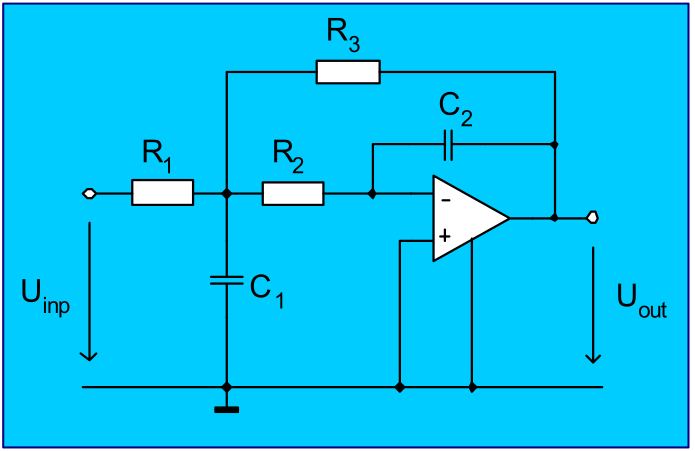
\includegraphics[width=0.7\linewidth]{Obrazky/AE1/MFBDP}
		\caption{ARC Dolná priepusť 2. rádu - Huelsman - MFB, multiple feedback}
		\label{fig:mfbdp}
	\end{subfigure}
	\begin{subfigure}[b]{0.45\textwidth}
		\centering
		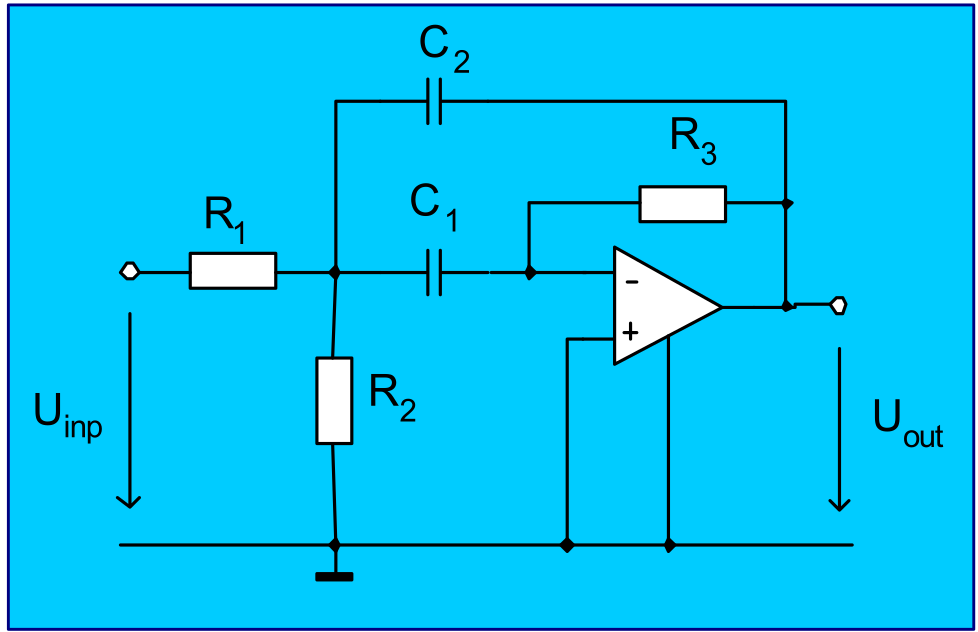
\includegraphics[width=0.7\linewidth]{Obrazky/AE1/MFBPP}
		\caption{ARC pásmová priepusť 2. rádu - Huelsman - MFB, multiple feedback}
		\label{fig:mfbPP}
	\end{subfigure}
	\caption{MFB topológie}
	\label{fig:mfb}
\end{figure}
Parametre \ref{fig:mfb} sa nedajú nezávisle nastavovať.
\begin{equation}
	\begin{aligned}
		K_0 = -\frac{R_3}{R_1} \,, \quad 
		\omega_p = \frac{1}{\sqrt{R_2 R_3 C_1 C_2}} \,, \quad 
		Q_p^{-1} = \sqrt{\frac{C_2}{C_1}} \left( \frac{\sqrt{R_2 R_3}}{R_1} + \sqrt{\frac{R_2}{R_3}} + \sqrt{\frac{R_3}{R_2}} \right) .
	\end{aligned}
\end{equation}
Úpravou MFB topológie \ref{fig:mfbdp} dosiahneme topológiu Sallen-Key, táto topológia má len jednu spätnú väzbu.
\begin{figure}[H]
	\centering
	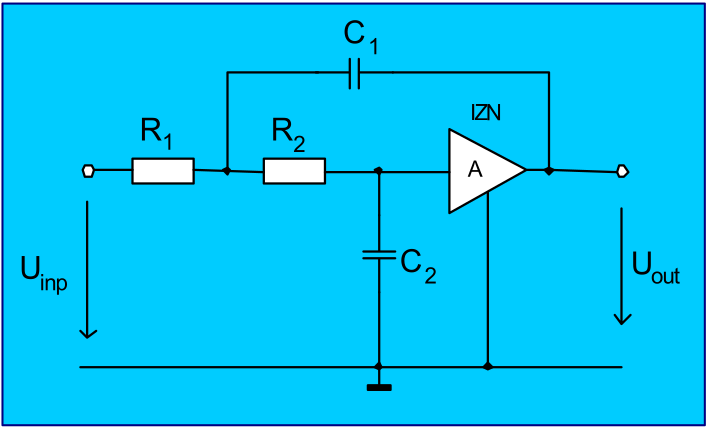
\includegraphics[width=0.4\linewidth]{Obrazky/AE1/sallenKeyDP}
	\caption{ARC 2. rádu dolná priepusť, Sallen-Key}
	\label{fig:sallenkeydp}
\end{figure}
Realizuje sa s neinvertujúcim zosilňovačom. V porovnaní s MFB je jednoduchšia. Obe topológie majú nízke citlivosti na komponenty. Aktívnu priepusť vieme realizovať zámenou R za C. R alebo C sa volia tak aby bolo $R_1 = R_2$ alebo $C_1 = C_2$. Nie však obe naraz.

\section{Aproximačné funkcie filtrov}
Aproximačná, alebo prenosová funkcia, plne popisuje správanie sa filtra v celej frekvenčnej oblasti. Aproximačná funkcia sa volí podľa požadovaného tolerančného kanálu - volí sa tak aby sa modul zmestil do nami definovaného poľa vo frekvenčnej oblasti.
Aproximačných funkcií existuje veľké množstvo, najpoužívanejšie sú uvedené nižšie.
\begin{figure}[H]
	\centering
	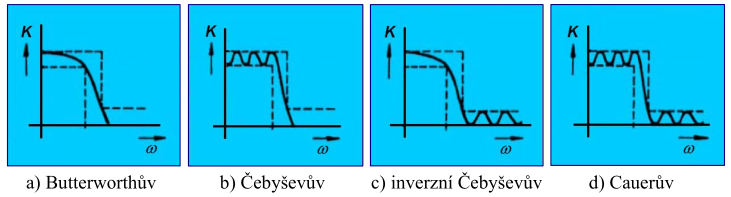
\includegraphics[width=0.7\linewidth]{Obrazky/AE1/aproximacneFunkcie}
	\caption{Bežne používané aproximačné funkcie.}
	\label{fig:aproximacnefunkcie}
\end{figure}
\begin{description}
	\item[Butterworth] Maximálne plochá prenosová charakteristika v priepustnom pásme, no nízka strmosť
	\item[Čebyšev] založené na izotermálnej aproximácií. Majú isté dovolené zvlnenie modulovej charakteristiky či už v priepustnom alebo nepriepustnom pásme (Inverzný Čebyšev)
	\item[Caurer] Dosahujú pri rovnakom ráde najvyššiu strmosť útlmu. Zvlnenie je aj priepustnom aj v nepriepustnom pásme. Nehodia sa pre prenos impulzov.
	\item[Bessel] Pre použitie s konštantným skupinovým oneskorením, majú maximálne lineárnu fázovú charakteristiku. 
\end{description}
\begin{figure}[H]
	\centering
	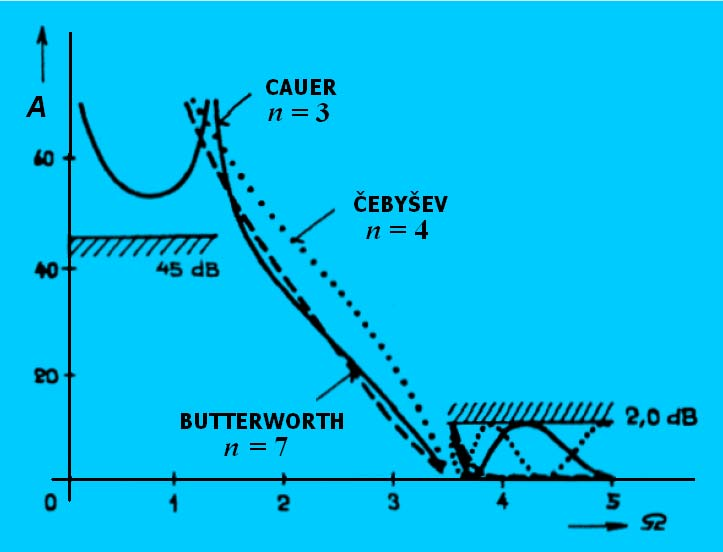
\includegraphics[width=0.4\linewidth]{Obrazky/AE1/porovnanieRadovFiltra}
	\caption{Porovnanie strmosti filtrov podľa rádu $n$}
	\label{fig:porovnanieradovfiltra}
\end{figure}
\section{Filtre vyšších rádov}
Filtre vyšších rádov sa realizujú formou kaskádneho zapojenia filtrov 2. a 1. rádu. V prípade pasívnych filtrov sa najčastejšie realizujú v podobe priečkovej štruktúry s rovnakou impedanciou na vstupe aj na výstupe. Pasívne filtre nie sú vhodné pre realizáciu vyšších rádov z dôvodu veľkosti, komplexnosti a ceny.

Kaskáda znamená súčin niekoľkých dielčich funkcií ktoré dokopy vytvoria funkciu vyššieho rádu. V praxi sa kaskáda navrhuje podľa návrhových tabuliek pre konkrétnu aproximačnú funkciu.

\chapter{Zosilňovače}
%Otázka - Zesilovače: kritéria pro klasifikaci, základní parametry, třídy zesilovačů, účinnost, širokopásmové zesilovače, úzkopásmové (laděné) zesilovače, výkonové (koncové) nf zesilovače. 

Základnou funkciou zosilňovača je zvýšiť užitočný výkon vstupného signálu - zväčší amplitúdu. Pričom by nemal akokoľvek pozmeniť časový priebeh vstupného signálu. Zosilňovače vykazujú stratový výkon. Poznáme jednočinné - ide len do plusu, a dvojčinné zosilňovače.
\section{Kritériá pre klasifikáciu zosilňovačov}
\begin{itemize}
	\item Podľa zosilovanej veličiny
	\begin{itemize}
		\item Zosilňovače napätia - $Z_{in} \rightarrow \text{max}$, $Z_{out} \rightarrow \text{min}$
		\item Zosilňovače prúdu - $Z_{in} \rightarrow \text{min}$, $Z_{out} \rightarrow \text{max}$
		\item Koncové zosilňovače - maximálny výstupný výkon
	\end{itemize}
	\item Podľa záťaže
	\begin{itemize}
		\item Rezistívna - nízkofrekvenčné zos.
		\item Kapacitna
		\item Induktívna - transformátor - koncové zos.
		\item rezonančný obvod - vf, nf zosilňovače
		\item Obezná impedancia
	\end{itemize}
	\item Podľa väzby vstupov
	\begin{itemize}
		\item priama, galvanická väzba - ss zos.
		\item odporová - ss, nf zos.
		\item kapacitná - striedavé zosilňovače
		\item transformátorová - koncové zosilňovače
		\item frekvenčne závislé články - korekčné zosilňovače
	\end{itemize}
	\item Podľa veľkosti vstupného signálu
	\begin{itemize}
		\item malý signál - lineárne zos.
		\item veľký signál - nelineárne zos.
	\end{itemize}
	\item Podľa pracovnej frekvencie
	\begin{itemize}
		\item jednosmerné - ss
		\item striedavé nf - audio
		\item striedavé vg - rádio
	\end{itemize}
	\item Podľa šírky pásma
	\begin{itemize}
		\item úzkopásmové - ladené vf
		\item širokopásmové - nf a vf
	\end{itemize}
	\item Podľa aktívneho prvku
	\begin{itemize}
		\item BJT
		\item FET
		\item Elektrónky
	\end{itemize}
	\item Podľa polohy pracovného bodu
	\begin{itemize}
		\item trieda A
		\item trieda B
		\item trieda AB
		\item trieda C
	\end{itemize}
\end{itemize}
\section{Parametre zosilňovačov}
Obdovodé funkcie \(K_U, \; K_I, \; K_P, \; Z_{inp}, \; Z_{out}\). \newline
Charakteristiky \(K(\omega), \; \varphi(\omega), \; u_{out}(u)_{in}\)
\begin{align}
	\underset{\text{Harmonické skreslenie}}{THD = \sqrt{\frac{U_2^2 + U_3^2 + \dots + U_n^2}{U_1^2 + U_2^2 + \dots + U_n^2}}}
	\qquad \quad 
	\underset{\text{(Gain Bandwidth Product)}}{GBP} = K_0 \cdot B 
	\qquad \quad 
	\underset{\text{Šumové číslo}}{F = \frac{\frac{P_{in}^{S}}{P_{in}^{N}}}{\frac{P_{out}^{S}}{P_{out}^{N}}}}
\end{align}
\section{Triedy zosilňovačov}
Existuje ich veľa, hlavné sú:
\begin{description}
	\item[Trieda A] Účinnosť malá, pod \qty{50}{\%}, používajú sa na malé signály. Minimálne skreslenie.
	\item[Trieda B] Účinnosť rádovo \qty{75}{\%}, dvojčinné zosilňovače, jedna vetva zosilňovača zosiluje kladnú a druhá zápornú pol-vlnu vstupného signálu
	\item[Trieda AB] Účinnosť podobne ako trieda B, dosahujú vyššie skreslenie, neprenášajú celú vlnu. Bežné v audiotechnike.
	\item[Trieda C] Teoretická účinnosť až \qty{100}{\%}. Extrémne miery skreslenia, používajú sa ako VF.
	\item[Trieda D] Jedná sa o digitálny zosilňovač ktorý na výstupe produkuje v podstate PWM. Skladá sa z generátora referenčného priebehu  a komparátora tohto priebehu s vstupným signálom.
\end{description}
\begin{figure}[H]
	\centering
	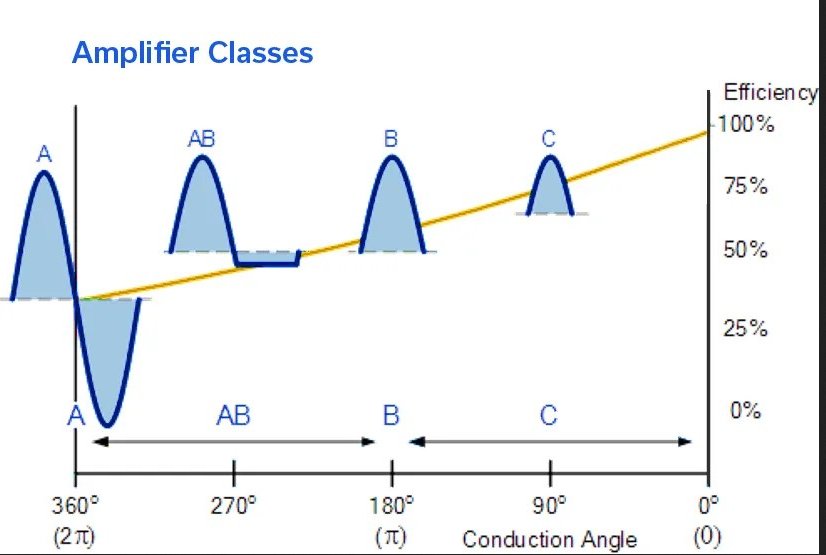
\includegraphics[width=0.4\linewidth]{Obrazky/AE1/TretiaOtazka/ZosilnovaceTriedy}
	\caption{Porovnanie výstupných priebeho základných tried zosilňovačov}
	\label{fig:zosilnovacetriedy}
\end{figure}
Trieda zosilňovača zároveň hovorí aj o jeho pracovnom bode. 
\begin{description}
	\item[Trieda A] Pracovný bod nastavený do stredu lineárnej časti charakteristiky
	\item[Trieda B] Pracovný bod je nastavený do bodu zániku kolektorového prúdu
	\item[Trieda C] Pracovný bod je nastavený hlboko do oblasti zániku kolektorového prúdu
	\item[Trieda AB] Pracovný bod je nastavený medzi stred lineárnej časti a bod zániku kolektorového prúdu
\end{description}
\section{Široko-pásmové zosilňovače}
Rozšíriť pásmo ktoré zosilňovač prenáša je možné výberom zapojenia (SC, SB, SE), využitím spätnej väzby, či modifikáciou zapojenia - delením záťaže.

Frekvenčne nezávislá spätná väzba - zložená z čiste rezistívnych komponentov, sa dá využiť tiež, jej využitie je v plyve zápornej spätnej väzby.
\begin{figure}[H]
	\centering
	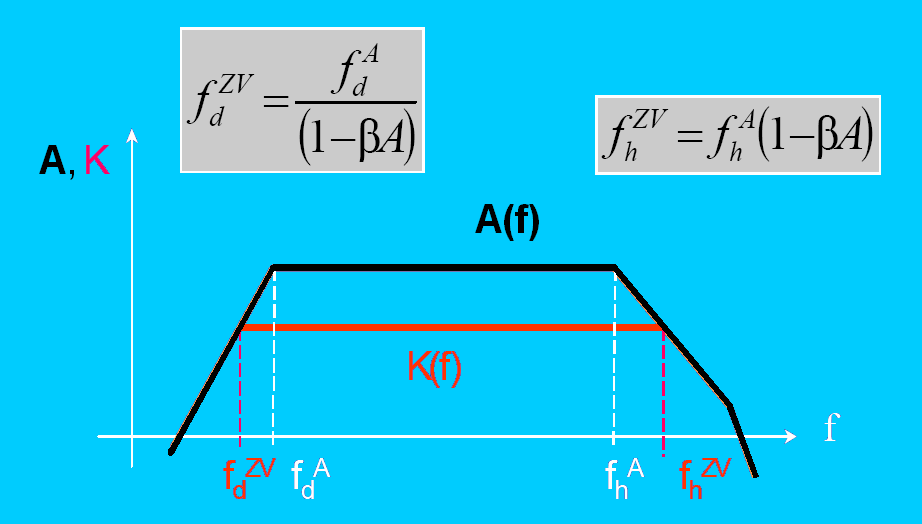
\includegraphics[width=0.4\linewidth]{Obrazky/AE1/TretiaOtazka/zapornaSpatnaVazba}
	\caption{Vplyv zápornej spätnej väzby na šírku pásma - teda medzné frekvencie.}
	\label{fig:zapornaspatnavazba}
\end{figure}

\begin{figure}[H]
	\centering
	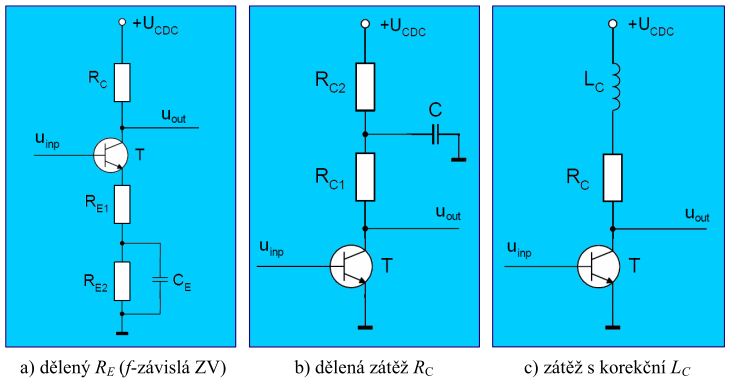
\includegraphics[width=0.7\linewidth]{Obrazky/AE1/TretiaOtazka/frekvenceZavislaVazba}
	\caption{Realizácia korekcie frek. char. formou závislej spätnej väzby}
	\label{fig:frekvencezavislavazba}
\end{figure}
Dá sa využiť aj frekvenčne závislá väzba \ref{fig:frekvencezavislavazba}. \ref{fig:frekvencezavislavazba}a - Kondenzátor $C_E$ sa vo vyšších frekvenciách skratuje, čo bude znamenať menšiu spätnú väzbu vo vyššom pásme. Rovnako to funguje aj pri \ref{fig:frekvencezavislavazba}b. Záťaž s korekčným $L_C$ nám zase poskytne v modulovej charakteristike rezonančné prevýšenie, keďže indukčnosť L tvorí s parazitnou kapacitou výstupu rezonančný obvod.

\section{Úzko-pásmové zosilňovače}
Jedná sa najmä o selektívne zosilňovače, ktoré zosilňujú len isté frekvencie. V malých výkonoch sa na tento účel používa trieda A v lineárnom režime. V závislosti od spôsobu napájania môže vyzerať principiálne zapojenie:
\begin{figure}[H]
	\centering
	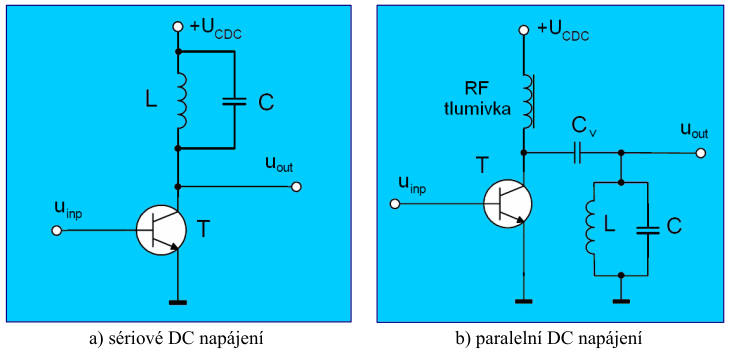
\includegraphics[width=0.6\linewidth]{Obrazky/AE1/TretiaOtazka/selektivnyZosi}
	\caption{Selektívny zosilňovač s jedným ladeným obvodom}
	\label{fig:selektivnyzosi}
\end{figure}
Selektívne zosilňovače mávajú rôzny parameter Q - Veľkosť prekmitu v charakteristike. Ladené obvody sa dajú rôzne pripájať a upravovať. Nakoľko toto nie je výkonový zosilňovač, tak to ešte musíme výkonovo zosilniť triedou C. Tá je pripojená k takémuto zosilňovaču odbočkou vytvorenou z autotransformátora.

VF zosilňovače sú náchylné na nestabilitu ktorá vzniká parazitnými kapacitami v tranzistore, ktoré odtlmia rezonančný obvod. Preto sa robí:
\begin{itemize}
	\item Neutralizácia zos. = opatrenie proti rozkmitaniu
	\item Unilaterizácia zos. = zabránenie spätného prenosu na vstup
\end{itemize}
\subsubsection{Výkonové úzko-pásmové}
Výkonové zosilňovače sa konštruujú z prvkov FET. Konštruujú sa v triede C. Pracujú ako koncové stupne, ktorých úlohou je zabezpečiť maximálny výstupný výkon, pracujú v nelineárnom režime. Pre veľmi veľké výkony sa stále používajú elektrónky.
\subsubsection{S viacerími ladenými obvodmi}
Dôvod využitia viacerých ladených obvodov môže byť zväčšenie šírky pásma. Ladené obvody pripájame na vstup a na výstup. Môžu byť ladené zhodne alebo aj nie.
\begin{figure}[H]
	\centering
	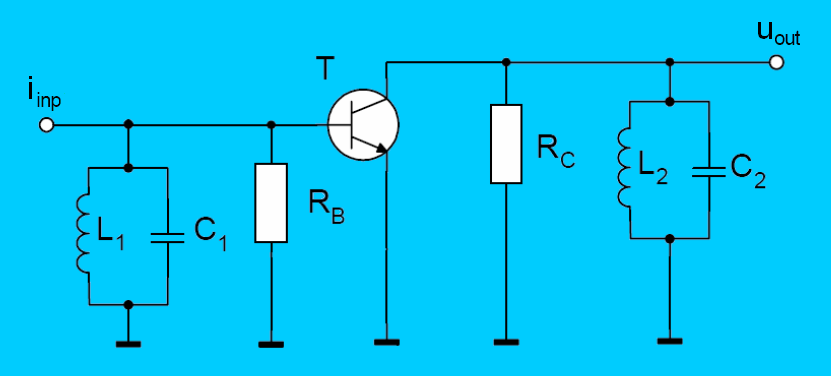
\includegraphics[width=0.4\linewidth]{Obrazky/AE1/TretiaOtazka/ZosikViacObvod1}
	\caption{Zosilňovač s viacerými ladenými obvodmi}
	\label{fig:zosikviacobvod}
\end{figure}

\begin{figure}[H]
	\centering
	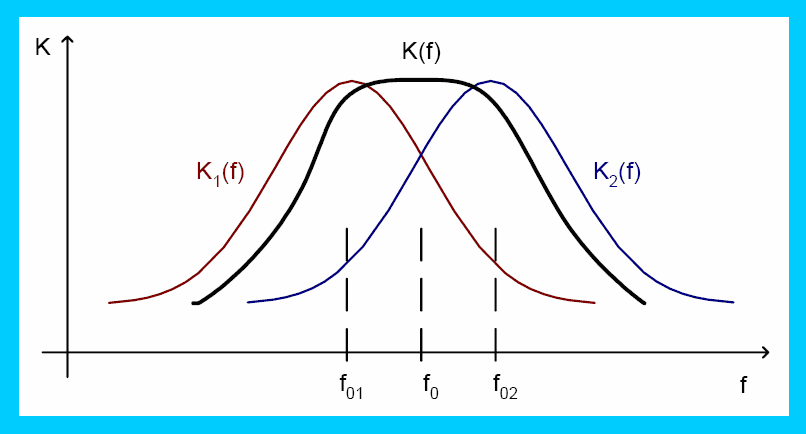
\includegraphics[width=0.4\linewidth]{Obrazky/AE1/TretiaOtazka/frekCharViacObvod}
	\caption{Frekvenčná charakteristika s viacerými ladenými obvodmi}
	\label{fig:frekcharviacobvod}
\end{figure}
Rozšírenie modulovej charakteristiky je možné použitím aj viazaného ladeného obvodu, založeného na indukčnosti - Induktívna väzba.
\section{Výkonové NF zosilňovače}
Výkonové zosilňovače sa realizujú v triedach A, B či AB. Majú poskytnúť maximálny akustický výkon, pričom sa hľadá optimálna záťaž pre maximálny výkon. Rozdelujú sa:
\begin{itemize}
	\item Podľa typu zapojenia
	\begin{itemize}
		\item SE
		\item SC
		\item Jednočinné / dvojčinné
	\end{itemize}
	\item Väzba medzi stupňami a záťažou
	\begin{itemize}
		\item Priama
		\item Kapacitná
		\item Transformátorová
	\end{itemize}
	\item Trieda
	\begin{itemize}
		\item Základné: A, B, AB, C
		\item Spínané: D, E, S, T, F, G, H
	\end{itemize}
\end{itemize}
Zosilňovač jednočinný v triede A s rezistívnou záťažou - používa sa minimálne, má účinnosť len  $25 \%$, no minimálne skreslenie. Pokiaľ nahradíme odpor $R_C$ transformátorom, dosiahneme účinnosti $50 \%$

Zosilňovač triedy B s transformátorom - obsahuje vstupný a výstupný transformátor. Teoretická hodnota účinnosti je $78.5\%$. Budiaci signál sa privádza fázovo posunutý na T1 a T2. 

Zosilňovač triedy B bez transformátora - nemá transformátor ani na vstupe ani na výstupe. 
\begin{figure}[H]
	\centering
	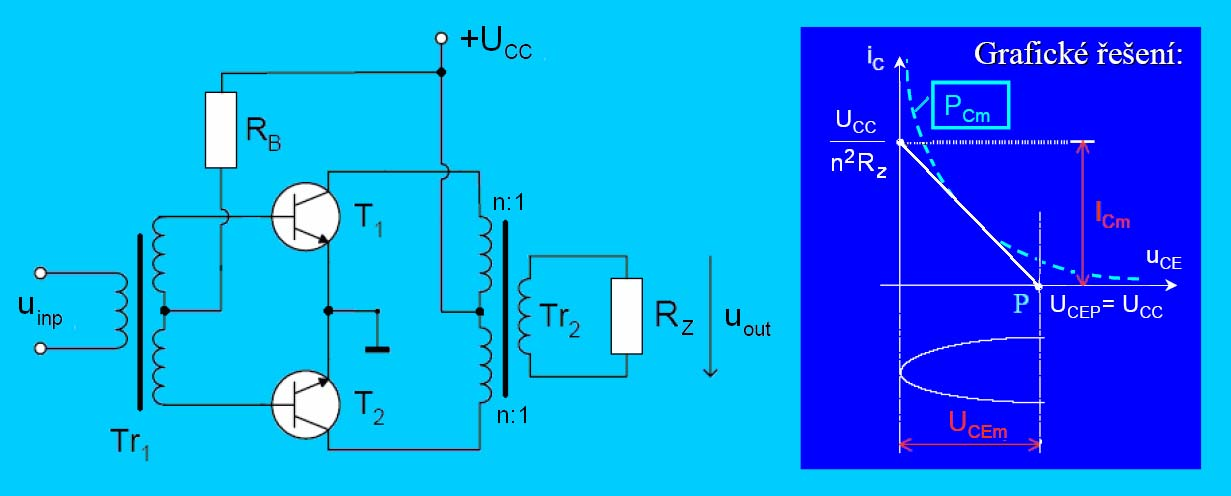
\includegraphics[width=0.7\linewidth]{Obrazky/AE1/TretiaOtazka/triedaBtransformator}
	\caption{NF zosilňovač triedy B s transformátormi}
	\label{fig:triedabtransformator}
\end{figure}
Zosilňovač triedy B bez transformátorov využíva fázový invertor miesto vstupného transformátora.
\begin{figure}[H]
	\centering
	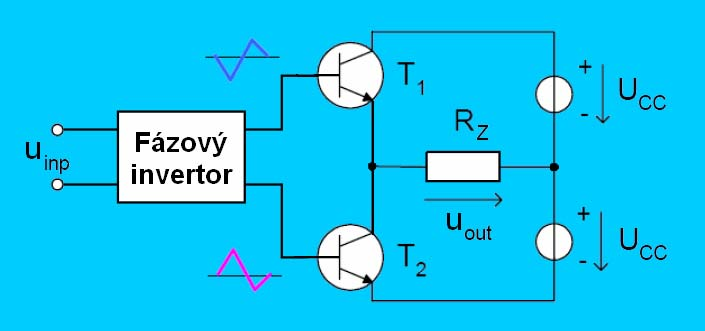
\includegraphics[width=0.7\linewidth]{Obrazky/AE1/TretiaOtazka/BbezTrafa}
	\caption{Zosilňovač triedy B bez transformátora.}
	\label{fig:bbeztrafa}
\end{figure}
\begin{figure}[H]
	\centering
	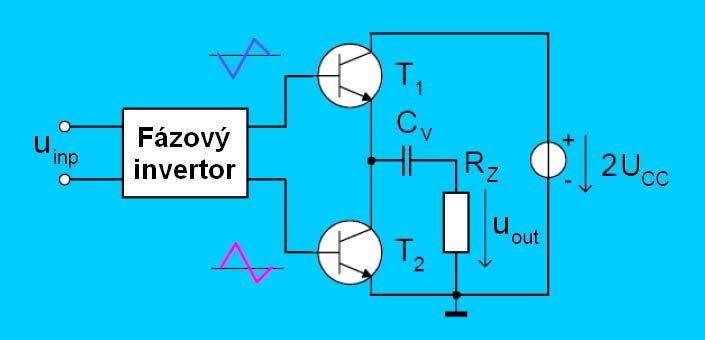
\includegraphics[width=0.7\linewidth]{Obrazky/AE1/TretiaOtazka/BbezTrafaDC}
	\caption{Zosilňovač triedy B s nesymetrickým zdrojom..}
	\label{fig:bbeztrafadc}
\end{figure}

V prípade, že sa použije nesymetrický DC zdroj, je potrebný väzobný kondenzátor na výstupe.

Dajú sa použiť aj komplementárne tranzistory, toto zjednoduší vstupnú budiacu časť. Používajú sa BJT tranzistory v pároch PNP a NPN.
\begin{figure}[H]
	\centering
	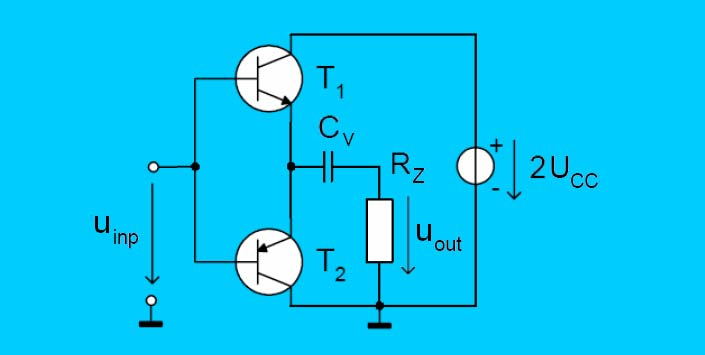
\includegraphics[width=0.7\linewidth]{Obrazky/AE1/TretiaOtazka/PNPNPNzosik}
	\caption{Zosilňovač triedy B s komplementárnym PNP NPN párom}
	\label{fig:pnpnpnzosik}
\end{figure}
Komplementárty pár musí mať rovnaké vlastnosti. Inak dochádza k skresleniu v oblasti prechodu nulou. Na potlačenie skreslenia sa používa napríklad trieda AB, resp. nastavenie kľudového pracovného bodu.

\begin{figure}[H]
	\centering
	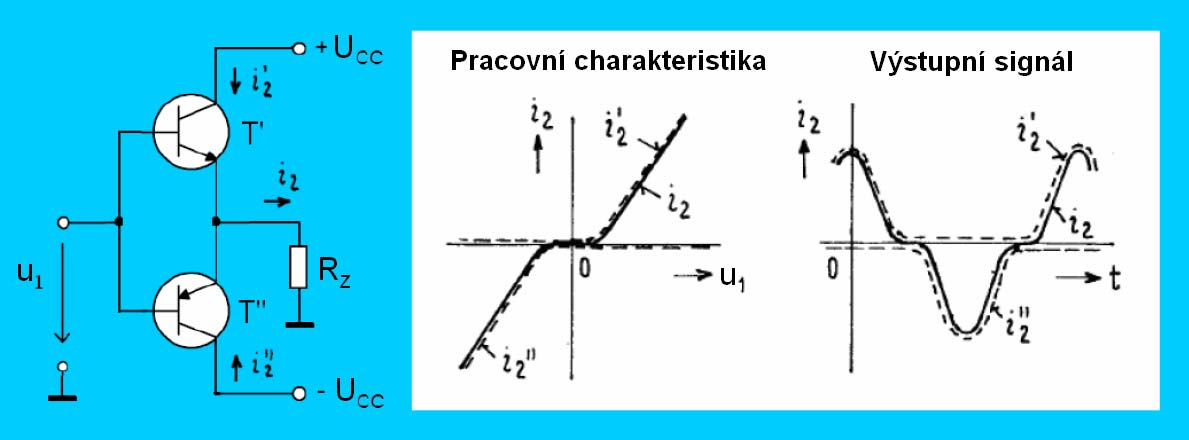
\includegraphics[width=0.7\linewidth]{Obrazky/AE1/TretiaOtazka/zkrelsenieB}
	\caption{Zkreslenie v komplementárnom zosilňovači triedy B}
	\label{fig:zkrelsenieb}
\end{figure}
\begin{figure}[H]
	\centering
	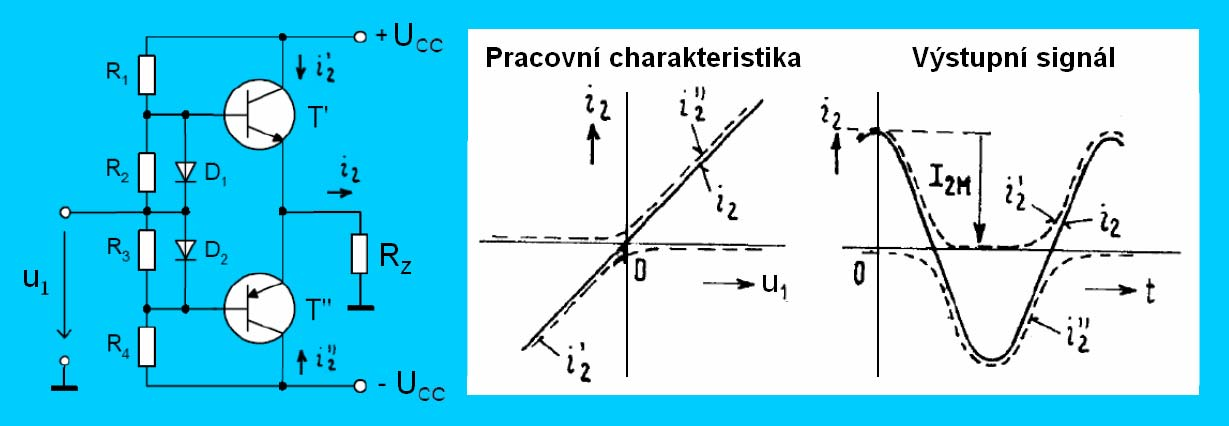
\includegraphics[width=0.7\linewidth]{Obrazky/AE1/TretiaOtazka/skreslenieAB}
	\caption{Trieda AB s komplementárnymi tranzistormi.}
	\label{fig:skreslenieab}
\end{figure}
\subsubsection{Spínané zosilňovače}
Spínaný zosilňovač sa realizuje s unipolárnymi tranzistormi. V podstate sa jedná o PWM generátor pripojený k výkonovému mostíku. Na výstup sa musí pripojiť LC filter.
\begin{figure}[H]
	\centering
	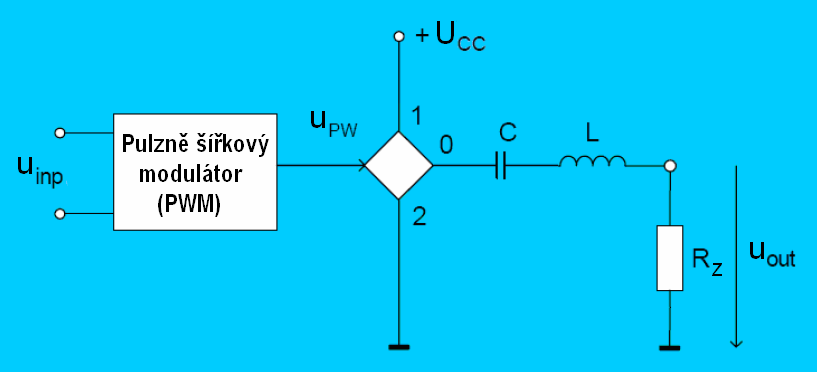
\includegraphics[width=0.7\linewidth]{Obrazky/AE1/TretiaOtazka/spinanyZosik}
	\caption{Spínaný zosilňovač}
	\label{fig:spinanyzosik}
\end{figure}


